\documentclass{article}           % Sets style/look of many things.
% \documentclass{report}          % part, chapters, front page etc.
\usepackage{exsheets}
\usepackage[utf8]{inputenc}       % Encoding of input files UTF-8
\usepackage[T1]{fontenc}
\usepackage[scaled]{beramono}     % Font
\usepackage{color}                % Color text
\usepackage{titlesec}             % Select alternative section titles
\usepackage{fancyvrb}
\usepackage{verbatim}             % Comment environment
\usepackage{listings}             % Format and render text/code etc.
\usepackage{minted}               % Much better syntax highlighting
\usepackage{float}                % Control of floating environment/figure
\usepackage{graphicx,  subfigure} % Better figures, graphics, units etc.
\usepackage{multicol}             % Multiple columns
\usepackage{amsmath}              % Math: Equation, split, align etc.
\usepackage{siunitx}              % SI units
\usepackage{mathtools}            % Different math tools to use with amsmath
\usepackage{amssymb}              % Math symbols
\usepackage[
    colorlinks,
    citecolor=black,              % I like links with standard black color
    filecolor=black,
    linkcolor=black,
    urlcolor=black
]{hyperref}                       % Links in TOC etc.
\usepackage[all]{hypcap}          % Better links to floating environment

\usepackage{tabto}
\newcommand\marginsymbol[1][0pt]{%
    \tabto*{0cm}\makebox[\dimexpr-1cm-#1\relax][r]{$\mathbb{P}$}\tabto*{\TabPrevPos}}

\renewcommand{\thesubsection}{\thesection.\alph{subsection}}

% Make margins smaller to fit more figures, tables etc on page: (optional)
\addtolength{\oddsidemargin}{-1.0in}
\addtolength{\evensidemargin}{-1.0in}
\addtolength{\textwidth}{2.0in}
\addtolength{\topmargin}{-0.8in}
\addtolength{\textheight}{1.6in}

\title{\vspace{-2cm}INF3490/INF4490 Exercise Solutions - Unsupervised Learning}
\author{Eivind Samuelsen\footnote{See \href{https://github.com/olehermanse/INF3490-AI_Machine_Learning/blob/master/README.md}{\textbf{README}} for complete list of authors/contributors.}
}
\date{}

% Removing paragraph indents is sometimes useful:
\setlength\parindent{0pt}
% ==============================================================================

% ================================= DOCUMENT ===================================
\begin{document}
    \renewcommand\marginsymbol[1][0pt]{%
  \tabto*{0cm}\makebox[-1cm][c]{$\mathbb{P}$}\tabto*{\TabPrevPos}}

\maketitle
\(\mathbb{P}\) marks the programming exercises, we strongly recommend using
the python programming language for these. Exercises may be added/changed
after publishing.


\section{k-means clustering}
The following graph shows 2D data points. It is clear from the graphs that there are two clusters. Will \(k\)-means clustering be able to find these two, if we define \(k = 2\)? If not, why?
\begin{figure}[H]
\begin{center}
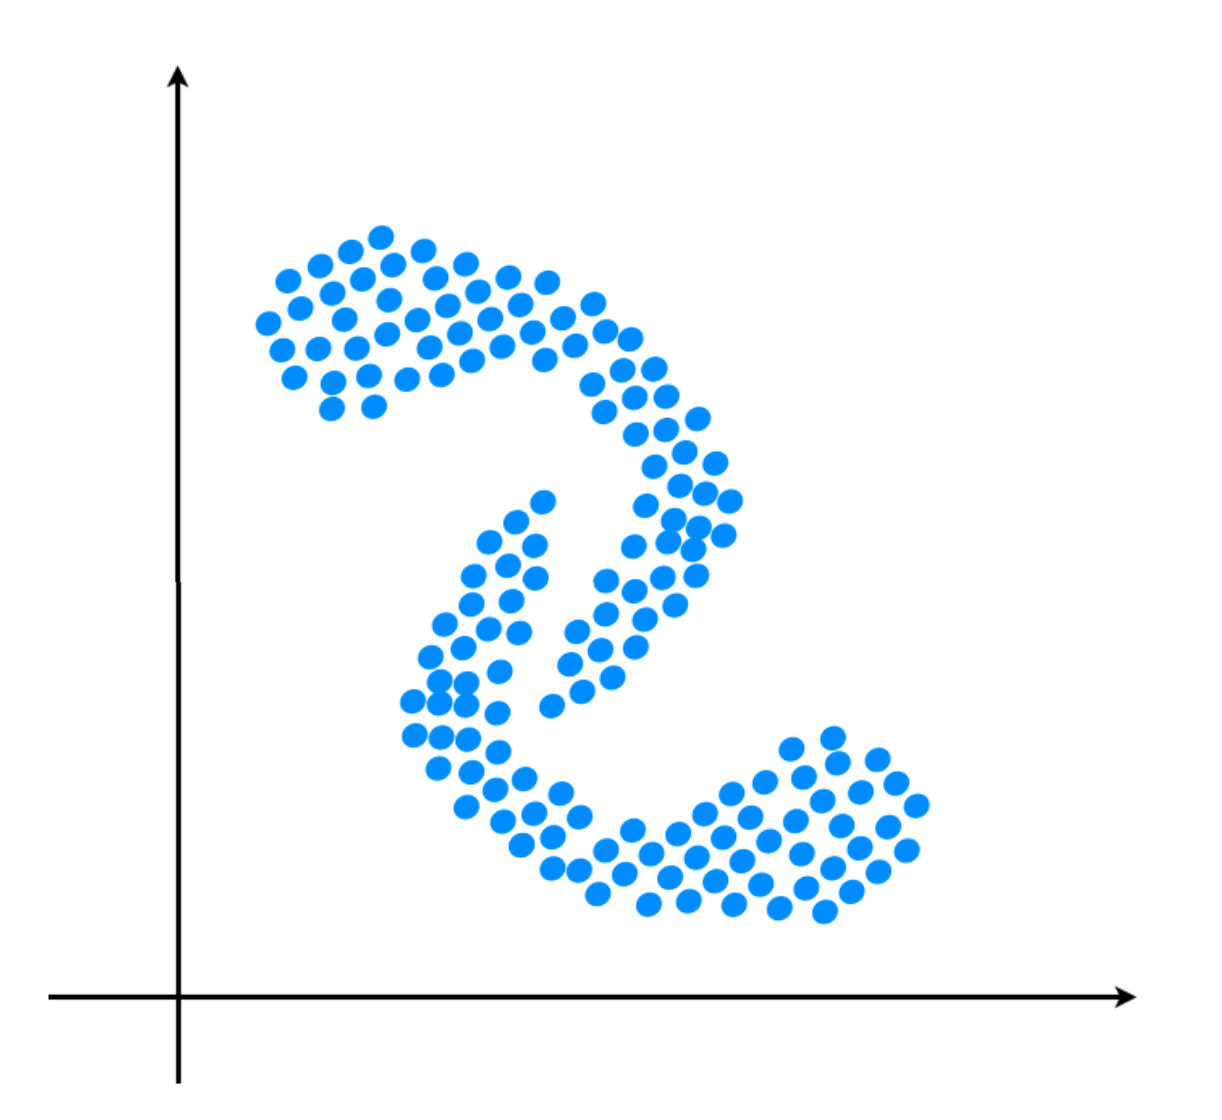
\includegraphics[width=0.6\textwidth]{two_clusters.png}
\end{center}
\end{figure}

\textit{Answer:}

\(k\)-means will struggle to find these clusters because they are non-convex shaped.
Some points (e.g. in the center of the graph) that lie in one cluster (from the two visibly obvious clusters) can be closer to the cluster center of the other cluster than the points in the other cluster.
The closeness between data points, since it is defined as the Euclidian distance, does not inform the k-means algorithm about the non-convex nature of the layout of these data points.

\section{Self organizing maps}
In SOMs, what role do the predefined topological (neighborhood) relationships between neurons in the map space play in the discovery of topological (neighborhood) relationships between input vectors in the data space?\\

\textit{Answer:}

The map layer defines a topological ordering over the neurons. The SOM algorithm works by making a map space neighbor neurons zone in on to similarities in the data space.
This is because the weights associated with all the map space neighbor neurons are moved towards the data points closest to the best matching neuron.
This makes weights of map space neighbor neurons adapt towards similar weights in the data space (weights having the same dimensionality as data, makes weight be elements of and move around in the data space).
Thus, similarities in the data are captured by map space neighbor neurons.
Visualization techniques are needed to see the dissimilarities in data space.
These techniques can allow seeing the separation between groups of neurons that represent different data clusters.

The relationship between map space and data space can be seen in the figure below.
The data points lying nearby the highlighted neuron (and its neighbordhood) in the data space (left hand side graph), will be represented by spatially close neurons in the map space (right hand side graph).

\begin{figure}[H]
\begin{center}
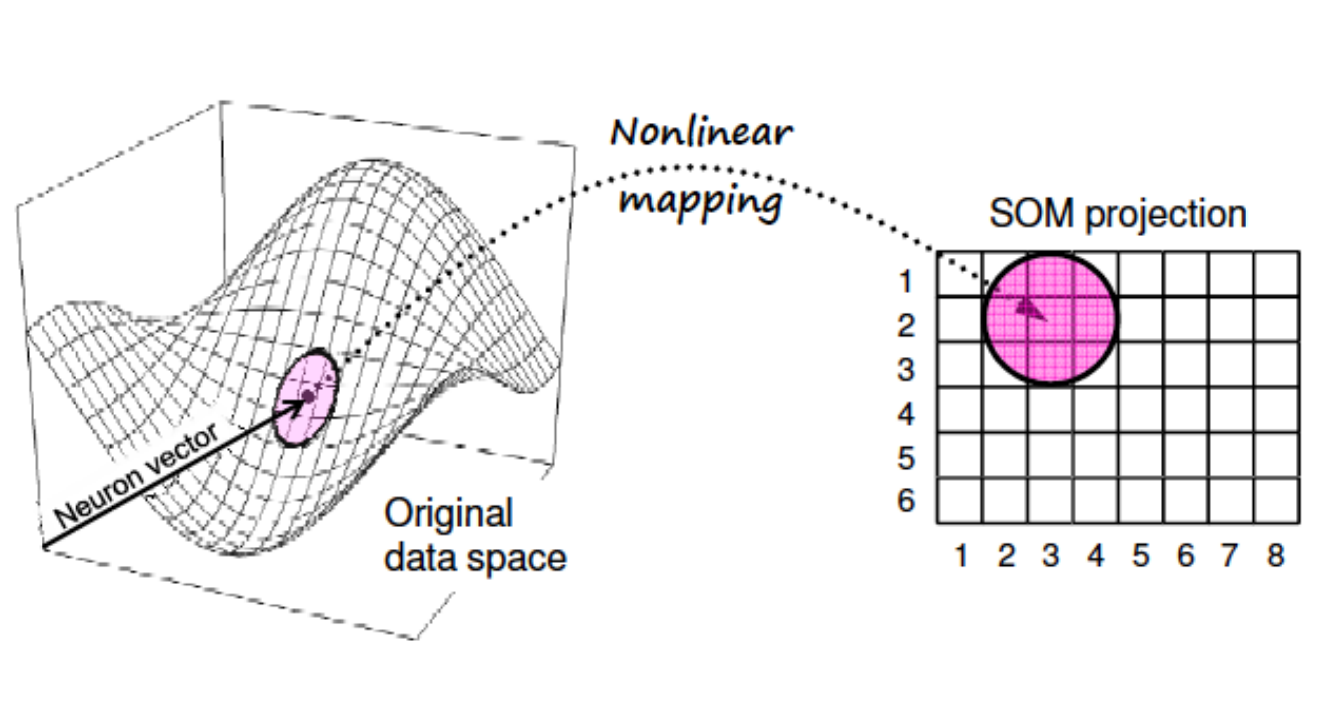
\includegraphics[width=0.9\textwidth]{spaces.png}
\end{center}
\end{figure}

Ideally, the winning and second place neurons will be close neighbors in the map space, because their weight vectors are similar.
Weight vectors that are similar are similar because they get adapted towards similar data points, i.e. points within some cluster.

\section{Gaussian function in SOMs}
In SOMs, a Gaussian function, as defined below, can be used to define the neighborhood relation
\begin{equation}
N(i,j) = e^{-\frac{||i-j||^2}{2\sigma^2(t)}}
\end{equation}
where \(i\) and \(j\) are two neurons, whose position on the lattice are given by (row, columnt), and \(||i-j||\) is the Euclidian distance between them. So, if \(i\)'s position is \((2,2)\) and \(j\)'s position is \((3,3)\) and \(\sigma(t) = 1\), \(N(i,j)\) will be \(e^{-1}\).

As can also be seen, the further a neuron \(i\) is from the winning neuron \(j\) on the lattice the smaller \(N(i,j)\) is. What would happen if \(N(i,j)\) is set to and remains zero for all neurons except the winning neuron? What would happen if \(N(i,j)\) is set to and remains 1 for all neurons including the winning neuron? Why is it important to have \(N(i,j)\) large for distant (on the lattice/map space) neurons in the beginning of the learning process i.e. \(j\) should have a larger neighborhood, and smaller as time goes by? This can be controlled by \(\sigma(t)=\sigma_0e^{-t/T}\), where \(\sigma_0\) is the initial value of \(\sigma\), and \(T\) is a constant.

Example Matlab script that can be run to see how the neighborhood funcion may change with time:
\begin{figure}[H]
\begin{center}
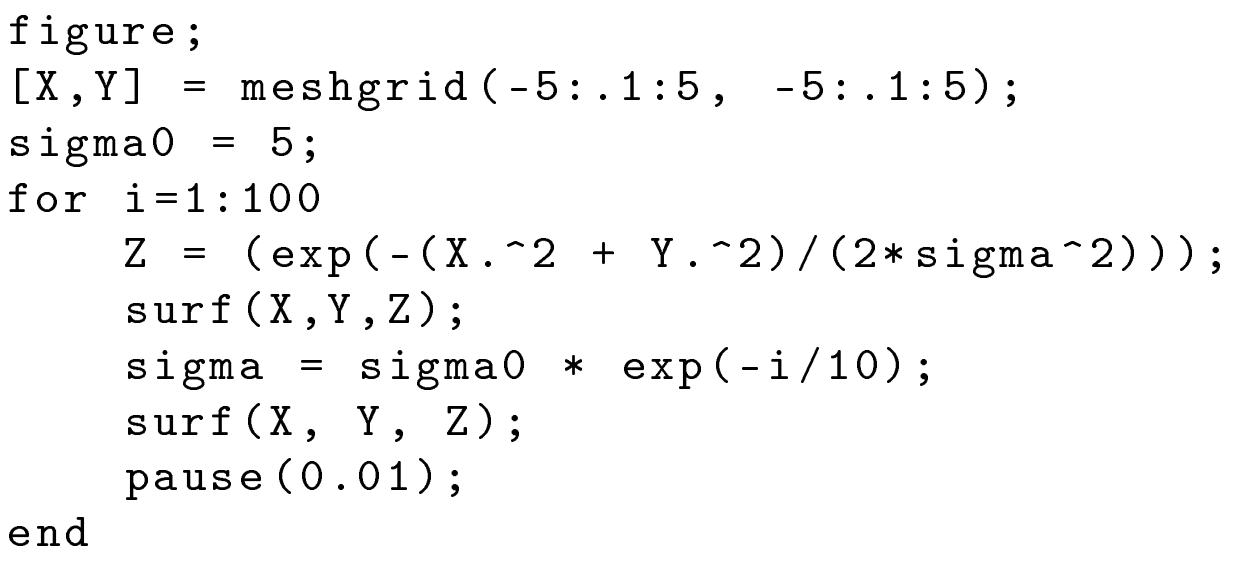
\includegraphics[width=0.6\textwidth]{matlab_example.png}
\end{center}
\end{figure}

Describe one other neighborhood relationship function that can be used for SOMs. In what way can it influence the learning process? Explain.\\

\textit{Answer:}

There are quite a few neighborhood relationship functions that have been investigated in SOM research.
In general, the neighborhood should be larger (somewhere half the size of the larger dimension in map space i.e. height or width of the map, whichever is greater) in size in the beginning of learning and gradually become smaller.
As long as such a reduction in time of the neighborhood is taken into consideration, different popular neighborhood functions lead to more or less similar learning results.

Typical functions other than Gaussian are:
\begin{itemize}
    \item \textbf{Bubble/flat function:} value is 1 up to a certain distance in the map neighborhood, otherwise 0.
    \begin{equation}
    N(i,j) =
    \begin{cases}
    1 & \text{if } ||i-j|| \leq \sigma \\
    0 & \text{otherwise}
    \end{cases}
    \end{equation}
    \item \textbf{Cut Gaussian function:} the Gaussian function is multiplied by the flat function so that it is smooth for close neurons and then cuts straight to zero at a certain distance:
    \begin{equation}
    N(i,j) =
    \begin{cases}
    e^{-\frac{||i-j||^2}{2\sigma^2(t)}}
      & \text{if } ||i-j|| \leq \sigma_{flat} \\
    0 & \text{otherwise}
    \end{cases}
    \end{equation}
    \item \textbf{Epanechicov function:} piecewise polynomial function is parabolic for near neighbors and zero above a certain distance:
    \begin{equation}
    N(i,j) =
    \max \Big\{0, 1 - (\frac{||i-j||}{\sigma})^2\Big\}
    \end{equation}

\end{itemize}

\section*{Contact and Github}
Corrections of grammar, language, notation or suggestions for improving this material are appreciated.
E-mail me at \href{mailto:olehelg@uio.no}{\textbf{olehelg@uio.no}} or use \href{https://github.com/olehermanse/INF3490-AI_Machine_Learning}{\textbf{GitHub}} to submit an issue or create a pull request.
The \href{https://github.com/olehermanse/INF3490-AI_Machine_Learning}{\textbf{GitHub repository}} contains all source code for assignments, exercises, solutions, examples etc.
As many people have been involved with writing and updating the course material, they are not all listed as authors here.
For a more complete list of authors and contributors see the \href{https://github.com/olehermanse/INF3490-AI_Machine_Learning/blob/master/README.md}{\textbf{README}}.

\end{document}
% ==============================================================================
